%===============================================================================
% LaTeX sjabloon voor de bachelorproef toegepaste informatica aan HOGENT
% Meer info op https://github.com/HoGentTIN/latex-hogent-report
%===============================================================================

\documentclass[dutch,dit,thesis]{hogentreport}

% TODO:
% - If necessary, replace the option `dit`' with your own department!
%   Valid entries are dbo, dbt, dgz, dit, dlo, dog, dsa, soa
% - If you write your thesis in English (remark: only possible after getting
%   explicit approval!), remove the option "dutch," or replace with "english".

\usepackage{lipsum} % For blind text, can be removed after adding actual content

%% Pictures to include in the text can be put in the graphics/ folder
\graphicspath{{graphics/}}

%% For source code highlighting, requires pygments to be installed
%% Compile with the -shell-escape flag!
\usepackage[section]{minted}
%% If you compile with the make_thesis.{bat,sh} script, use the following
%% import instead:
%% \usepackage[section,outputdir=../output]{minted}
\usemintedstyle{solarized-light}
\definecolor{bg}{RGB}{253,246,227} %% Set the background color of the codeframe

%% Change this line to edit the line numbering style:
\renewcommand{\theFancyVerbLine}{\ttfamily\scriptsize\arabic{FancyVerbLine}}

%% Macro definition to load external java source files with \javacode{filename}:
\newmintedfile[javacode]{java}{
    bgcolor=bg,
    fontfamily=tt,
    linenos=true,
    numberblanklines=true,
    numbersep=5pt,
    gobble=0,
    framesep=2mm,
    funcnamehighlighting=true,
    tabsize=4,
    obeytabs=false,
    breaklines=true,
    mathescape=false
    samepage=false,
    showspaces=false,
    showtabs =false,
    texcl=false,
}

% Other packages not already included can be imported here

%%---------- Document metadata -------------------------------------------------
% TODO: Replace this with your own information
\author{Lode Van Beneden}
\supervisor{Mevr. C. De Leenheer}
\cosupervisor{Mr. A. Hantson}
\title[Optionele ondertitel]%
    {In hoeverre kan kunstmatige intelligentie worden in-gezet om vermoeidheid bij automobilisten te detecte-ren en signaleren, en welke maatregelen zouden kun-nen worden geïmplementeerd om ongevallen te voor-komen?}
\academicyear{\advance\year by -1 \the\year--\advance\year by 1 \the\year}
\examperiod{1}
\degreesought{\IfLanguageName{dutch}{Professionele bachelor in de toegepaste informatica}{Bachelor of applied computer science}}
\partialthesis{false} %% To display 'in partial fulfilment'
%\institution{Internshipcompany BVBA.}

%% Add global exceptions to the hyphenation here
\hyphenation{back-slash}

%% The bibliography (style and settings are  found in hogentthesis.cls)
\addbibresource{bachproef.bib}            %% Bibliography file
\addbibresource{../voorstel/voorstel.bib} %% Bibliography research proposal
\defbibheading{bibempty}{}

%% Prevent empty pages for right-handed chapter starts in twoside mode
\renewcommand{\cleardoublepage}{\clearpage}

\renewcommand{\arraystretch}{1.2}

%% Content starts here.
\begin{document}

%---------- Front matter -------------------------------------------------------

\frontmatter

\hypersetup{pageanchor=false} %% Disable page numbering references
%% Render a Dutch outer title page if the main language is English
\IfLanguageName{english}{%
    %% If necessary, information can be changed here
    \degreesought{Professionele Bachelor toegepaste informatica}%
    \begin{otherlanguage}{dutch}%
        \maketitle%
    \end{otherlanguage}%
}{}

%% Generates title page content
\maketitle
\hypersetup{pageanchor=true}

%%=============================================================================
%% Voorwoord
%%=============================================================================

\chapter*{\IfLanguageName{dutch}{Woord vooraf}{Preface}}%
\label{ch:voorwoord}
\setlength{\parskip}{1em}
%% TODO:
%% Het voorwoord is het enige deel van de bachelorproef waar je vanuit je
%% eigen standpunt (``ik-vorm'') mag schrijven. Je kan hier bv. motiveren
%% waarom jij het onderwerp wil bespreken.
%% Vergeet ook niet te bedanken wie je geholpen/gesteund/... heeft
Geachte lezer,

Met veel genoegen presenteer ik mijn bachelorproef, met de titel "In hoeverre kan kunstmatige intelligentie worden in-gezet om vermoeidheid bij automobilisten te detecteren en signaleren, en welke maatregelen zouden kunnen worden geïmplementeerd om ongevallen te voorkomen?".
Dit onderzoek is het resultaat van mijn toewijding aan het vakgebied van kunstmatige intelligentie.

De keuze voor dit onderwerp werd beslist door mijn interesse in de opkomst van kunstmatige intelligentie en de bezorgdheid over het gevaarlijk rijgedrag van sommige automobilisten. In dit voorwoord
wil ik kort de achtergrond van mijn onderzoek uitleggen en mijn dank uitspreken aan degene die mij hebben geholpen aan het tot stand komen van dit werk.

Mijn oprechte dank gaat uit naar mijn begeleider, Alec Hantson, voor de waardevolle begeleiding en ondersteuning gedurende dit onderzoeksproces. Zijn expertise op het vakgebied van kunstmatige intelligentie heeft mij veel begrip en inzicht gegeven.
Ook wil ik mijn promotor, Chloé De Leenheer, bedanken die mij ondersteunt en begeleidt heeft om dit werk zo correct en professioneel mogelijk te verwoorden.

Dit onderzoek heeft niet enkel mijn academische vaardigheid verbreedt, maar heeft mij ook bewust gemaakt op de impact die kunstmatige intelligentie kan hebben op maatschappelijke kwesties zoals verkeersveiligheid.
Ik hoop dat de resultaten en aanbevelingen in deze bachelorproef bijdragen aan de rol van technologie in het verkeerd.

Ik nodig u uit om de pagina's van dit werk te verkennen en hoop dat dit u een inzicht geeft in de relatie tussen kunstmatige intelligentie, vermoeidheid bij automobilisten en verkeersveiligheid.
Hopelijk draagt dit onderzoek bij aan een veiligere en slimmere mobiliteit in het verkeer in de toekomst.

Met vriendelijke groet,

Lode Van Beneden
\\
Bachelor Toegepaste informatica
\\
Hogeschool Gent
%%=============================================================================
%% Samenvatting
%%=============================================================================

% TODO: De "abstract" of samenvatting is een kernachtige (~ 1 blz. voor een
% thesis) synthese van het document.
%
% Een goede abstract biedt een kernachtig antwoord op volgende vragen:
%
% 1. Waarover gaat de bachelorproef?
% 2. Waarom heb je er over geschreven?
% 3. Hoe heb je het onderzoek uitgevoerd?
% 4. Wat waren de resultaten? Wat blijkt uit je onderzoek?
% 5. Wat betekenen je resultaten? Wat is de relevantie voor het werkveld?
%
% Daarom bestaat een abstract uit volgende componenten:
%
% - inleiding + kaderen thema
% - probleemstelling
% - (centrale) onderzoeksvraag
% - onderzoeksdoelstelling
% - methodologie
% - resultaten (beperk tot de belangrijkste, relevant voor de onderzoeksvraag)
% - conclusies, aanbevelingen, beperkingen
%
% LET OP! Een samenvatting is GEEN voorwoord!

%%---------- Nederlandse samenvatting -----------------------------------------
%
% TODO: Als je je bachelorproef in het Engels schrijft, moet je eerst een
% Nederlandse samenvatting invoegen. Haal daarvoor onderstaande code uit
% commentaar.
% Wie zijn bachelorproef in het Nederlands schrijft, kan dit negeren, de inhoud
% wordt niet in het document ingevoegd.

\IfLanguageName{english}{%
\selectlanguage{dutch}
\chapter*{Samenvatting}
\lipsum[1-4]
\selectlanguage{english}
}{}

%%---------- Samenvatting -----------------------------------------------------
% De samenvatting in de hoofdtaal van het document

\chapter*{\IfLanguageName{dutch}{Samenvatting}{Abstract}}

\lipsum[1-4]


%---------- Inhoud, lijst figuren, ... -----------------------------------------

\tableofcontents

% In a list of figures, the complete caption will be included. To prevent this,
% ALWAYS add a short description in the caption!
%
%  \caption[short description]{elaborate description}
%
% If you do, only the short description will be used in the list of figures

\listoffigures

% If you included tables and/or source code listings, uncomment the appropriate
% lines.
%\listoftables
%\listoflistings

% Als je een lijst van afkortingen of termen wil toevoegen, dan hoort die
% hier thuis. Gebruik bijvoorbeeld de ``glossaries'' package.
% https://www.overleaf.com/learn/latex/Glossaries

%---------- Kern ---------------------------------------------------------------

\mainmatter{}

% De eerste hoofdstukken van een bachelorproef zijn meestal een inleiding op
% het onderwerp, literatuurstudie en verantwoording methodologie.
% Aarzel niet om een meer beschrijvende titel aan deze hoofdstukken te geven of
% om bijvoorbeeld de inleiding en/of stand van zaken over meerdere hoofdstukken
% te verspreiden!

%%=============================================================================
%% Inleiding
%%=============================================================================

\chapter{\IfLanguageName{dutch}{Inleiding}{Introduction}}%
\label{ch:inleiding}

De inleiding moet de lezer net genoeg informatie verschaffen om het onderwerp te begrijpen en in te zien waarom de onderzoeksvraag de moeite waard is om te onderzoeken. In de inleiding ga je literatuurverwijzingen beperken, zodat de tekst vlot leesbaar blijft. Je kan de inleiding verder onderverdelen in secties als dit de tekst verduidelijkt. Zaken die aan bod kunnen komen in de inleiding~\autocite{Pollefliet2011}:

\begin{itemize}
  \item context, achtergrond
  \item afbakenen van het onderwerp
  \item verantwoording van het onderwerp, methodologie
  \item probleemstelling
  \item onderzoeksdoelstelling
  \item onderzoeksvraag
  \item \ldots
\end{itemize}

\section{\IfLanguageName{dutch}{Probleemstelling}{Problem Statement}}%
\label{sec:probleemstelling}

Uit je probleemstelling moet duidelijk zijn dat je onderzoek een meerwaarde heeft voor een concrete doelgroep. De doelgroep moet goed gedefinieerd en afgelijnd zijn. Doelgroepen als ``bedrijven,'' ``KMO's'', systeembeheerders, enz.~zijn nog te vaag. Als je een lijstje kan maken van de personen/organisaties die een meerwaarde zullen vinden in deze bachelorproef (dit is eigenlijk je steekproefkader), dan is dat een indicatie dat de doelgroep goed gedefinieerd is. Dit kan een enkel bedrijf zijn of zelfs één persoon (je co-promotor/opdrachtgever).

\section{\IfLanguageName{dutch}{Onderzoeksvraag}{Research question}}%
\label{sec:onderzoeksvraag}

Wees zo concreet mogelijk bij het formuleren van je onderzoeksvraag. Een onderzoeksvraag is trouwens iets waar nog niemand op dit moment een antwoord heeft (voor zover je kan nagaan). Het opzoeken van bestaande informatie (bv. ``welke tools bestaan er voor deze toepassing?'') is dus geen onderzoeksvraag. Je kan de onderzoeksvraag verder specifiëren in deelvragen. Bv.~als je onderzoek gaat over performantiemetingen, dan 

\section{\IfLanguageName{dutch}{Onderzoeksdoelstelling}{Research objective}}%
\label{sec:onderzoeksdoelstelling}

Wat is het beoogde resultaat van je bachelorproef? Wat zijn de criteria voor succes? Beschrijf die zo concreet mogelijk. Gaat het bv.\ om een proof-of-concept, een prototype, een verslag met aanbevelingen, een vergelijkende studie, enz.

\section{\IfLanguageName{dutch}{Opzet van deze bachelorproef}{Structure of this bachelor thesis}}%
\label{sec:opzet-bachelorproef}

% Het is gebruikelijk aan het einde van de inleiding een overzicht te
% geven van de opbouw van de rest van de tekst. Deze sectie bevat al een aanzet
% die je kan aanvullen/aanpassen in functie van je eigen tekst.

De rest van deze bachelorproef is als volgt opgebouwd:

In Hoofdstuk~\ref{ch:stand-van-zaken} wordt een overzicht gegeven van de stand van zaken binnen het onderzoeksdomein, op basis van een literatuurstudie.

In Hoofdstuk~\ref{ch:methodologie} wordt de methodologie toegelicht en worden de gebruikte onderzoekstechnieken besproken om een antwoord te kunnen formuleren op de onderzoeksvragen.

% TODO: Vul hier aan voor je eigen hoofstukken, één of twee zinnen per hoofdstuk

In Hoofdstuk~\ref{ch:conclusie}, tenslotte, wordt de conclusie gegeven en een antwoord geformuleerd op de onderzoeksvragen. Daarbij wordt ook een aanzet gegeven voor toekomstig onderzoek binnen dit domein.
\chapter{\IfLanguageName{dutch}{Stand van zaken}{State of the art}}%
\label{ch:stand-van-zaken}

% Tip: Begin elk hoofdstuk met een paragraaf inleiding die beschrijft hoe
% dit hoofdstuk past binnen het geheel van de bachelorproef. Geef in het
% bijzonder aan wat de link is met het vorige en volgende hoofdstuk.

% Pas na deze inleidende paragraaf komt de eerste sectiehoofding.
Om dit onderzoek tot stand te brengen, is er nood aan bepaalde informatie, waaronder over AI-technieken en vermoeidheid zelf. Nadien wordt dit alles verwerkt om het probleem aan te pakken.

\section{Vermoeidheid}
De verkeersveiligheid heeft een grote last van vermoeidheid en slaperigheid. In de literatuur is de definitie van vermoeidheid en slaperigheid anders en bestaat er eigenlijk geen duidelijk onderscheid tussen beide \autocite{RiguelleGoldenbeld}.

Vermoeidheid verwijst naar een weerstand die veroorzaakt wordt door uitputting. Dit heeft het gevolg dat de taken minder efficiënt worden uitgevoerd. Dit kan zowel fysiek (bijvoorbeeld na het sporten of intensief werken) als mentaal zijn (na een veeleisende intellectuele, mentale of psychologische activiteit). Vermoeidheid zorgt er voor dat de taak minder snel wordt afgemaakt of dat de energie zodanig laag ligt dat er aan de volgende taak niet begonnen wordt.

Slaperigheid verwijst naar de moeite om nog wakker te blijven. Het is gekoppeld aan de biologische slaap-waak proces volgens het circadiaan-ritme. Het circadiaan-ritme is een endogene, regelbare schommeling van ongeveer 24 uur (van Latijnse `circa-diem` - ongeveer een dag) van verschillende biologische systemen in het hele lichaam \autocite{Gianni2018}. Slaperigheid heeft dus geen rechtstreeks verband met de uitvoering van een activiteit. Doordat ons menselijk lichaam beschikt over een 'slaapmodus', dit is voornamelijk tussen middernacht en 6 uur, neemt de alertheid bijgevolg af. Dit komt doordat het lichaam, op een cyclus van 24 uur, meer slaap nodig heeft dan op andere momenten.

Hoewel slaperigheid en vermoeidheid logisch niet synchroon verlopen, worden ze vaak gezamenlijk behandeld in de literatuur vanwege hun overeenkomstige gevolgen. Deze twee aparte gevallen kunnen ook tegelijkertijd voorkomen bij iemand. Om het eenvoudig te houden, wordt 'vermoeidheid' waargenomen als slaperigheid.

\section{Oorzaken van vermoeidheid}
Er zijn vijf algemene factoren, namelijk: de tijd besteed aan een taak of werk, slaaptekort, bioritme, monotonie van een taak en individuele kenmerken, die vermoeidheid veroorzaken \autocite{Brown}.
\subsection{De tijd besteed aan een taak of werk}
Eén van de mogelijke oorzaken is de tijd die iemand besteed aan een bepaalde taak of werk. De meeste mensen voelen de eerste symptomen van fysieke vermoeidheid na ongeveer 2 à 3 uren aaneengesloten autorijden \autocite{RiguelleGoldenbeld}.
\subsection{Slaaptekort}
Een slaaptekort kan chronisch of acuut zijn \autocite{VanSchagen2003}. Een chronisch slaaptekort kan veroorzaakt worden door gevolg van te weinig slaap over een lange periode. Men heeft gemiddeld nood aan 8 uur slaap. Echter is het ook van belang dat er goed geslapen wordt. Er kunnen regelmatige verstoringen optreden tijdens het slapen, wat ook leidt tot een chronisch slaaptekort. Een acuut slaaptekort komt ook door het te weinig slapen, maar is minder structureel. Na één slechte of korte nacht, wordt er al gesproken van een partieel acuut slaaptekort. Een volledig acuut slaaptekort komt pas voor indien er in de gehele 24-uursperiode niet geslapen is.
\subsection{Bioritme}
Het bioritme regelt het slaap-waakritme van de mens. Dit is bij iedereen anders. Het hangt dus samen met de dagelijkse slaapcyclus. Dit betekent dat de mens in de ochtend minder behoefte heeft aan slaapt dan op andere tijdstippen. Wanneer de tijd richting middernacht gaat, zal het bioritme meer nood hebben aan slaap. Soms zit er geen consistentie in het bioritme, bijvoorbeeld wanneer iemand nachtdienst heeft.
\subsection{Monotonie van de taak}
Vermoeidheid kan zich ook vormen doordat men een monotone taak uitvoert. Een taak is monotoon wanneer prikkels ontbreken, verandering erg voorspelbaar is of er een hoge maat van herhaling is \autocite{DaCoTA}. Het rijden op een autosnelweg met weinig verkeer en verandering van omgeving kan men zien als een monotone taak. Uit een experimenteel onderzoek is ook gebleken dat de monotonie van een rijtaak na verloop van tijd tot een slechtere rijprestatie leidt.
\subsection{Individuele kenmerken}
Tenslotte hebben individuele kenmerken ook een invloed op de vermoeidheid. Deze factoren, zoals leeftijd, medische conditie, het gebruik van alcohol, geneesmiddelen of drugs, beïnvloeden hoe vatbaar iemand is voor vermoeidheid en hoe goed ze er mee kunnen omgaan \autocite{VanSchagen2003}. Zo zijn oudere mensen, die last hebben van een slechte lichamelijke conditie, vaak sneller vermoeid. In tegenstelling tot tieners, die extra vatbaar zijn voor vermoeidheidseffecten door alcohol, drugs en te weinig slaap.

\section{Verband met verkeersveiligheid}
\subsection{Invloed op het rijgedrag}
Het effect van vermoeidheid op verkeersveiligheid is in verschillende studies onderzocht. Volgens deze studies leidt vermoeidheid achter het stuur tot een aantal negatieve effecten op verkeersgedrag \autocite{RiguelleGoldenbeld}. Deze bestaan uit een tragere reactietijd, verminderende oplettendheid en verwerking van informatie en slechter sturen \autocite{Bartlett,Friswell2008}. 

Volgens onderzoek is de rijprestatie van bestuurders na 17-19 uur slaapdeprivatie slechter dan die van bestuurders met een BAC (bloed-alcohol percentage) van 0.5\%, wat de wettelijke grens is in de meeste Europese landen en Australië \autocite{Williamson2000}. Onderzoek van Dawson \& Reid (1997) geeft aan dat de rijprestatie afneemt na 16 uur slaapdeprivatie en dat 21 uur leidt tot een verminderde rijprestatie die gelijk is aan een BAC van 0.8\%, wat het wettelijk limiet is in Engeland, de Verenigde Staten en Canada \autocite{Dawson1997}.
\subsection{Gevolgen in termen van ongevallen}
De prevalentie van vermoeidheid en de impact dat het heeft op ongevallen, is niet makkelijk te meten \autocite{Diependaele2015}. Dit komt doordat er geen betrouwbaar meetprotocol bestaat. Mensen die in een ongeval terecht komen, geven vaak ook niet toe dat het door de vermoeidheid komt dat het heeft plaatsgevonden. De gegevens uit het "100 Car Naturalistic Driving"-onderzoek tonen aan dat rijden als men moe is, leidt tot een vier keer meer risico op een ongeval \autocite{Klauer2006}.

Wetenschappelijke schattingen, gebaseerd op diepgaande analyses van de verkeersongevallen, geven aan dat 10 tot 15\% van de ongevallen te maken zou hebben met vermoeidheid \autocite{VanSchagen2003}. Een andere schatting zegt dat ongeveer 20 tot 25\% van de ongevallen op Europese wegen te maken heeft met vermoeidheid \autocite{Akerstedt2013}. \textcite{Horne1995} schatten dat vermoeidheid de oorzaak is van 16\% voor de ongevallen op stadswegen en 20\% op autosnelwegen. Een recentere studie van dezelfde auteurs \autocite{Horne1999} bevestigt dat de ongevallen door middel van vermoeidheid vaker gebeuren op autosnelwegen doordat rijden op een autosnelweg gezien wordt als een monotone taak. 
Gebleken uit een analyse van over 600 ongevallen met vrachtwagens in Europa blijkt dat vermoeidheid de hoofdoorzaak is van 6\% van de geanalyseerde ongevallen, waarvan maar liefst 37\% dodelijke ongevallen zijn \autocite{IRU2007}.

In België heeft een analyse van 125 letselongevallen met bussen of vrachtwagens aangetoond dat 10\% van de ongevallen veroorzaakt zijn door vermoeidheid \autocite{Herdewyn2010}. De Belgische ongevallenstatistieken van 2013 tonen aan dat het om 15.1\% van de verkeersongevallen om eenzijdige ongevallen, tegen een obstakel dat buiten de rijweg lag, ging. Hieruit kan er vermoed worden dat het om vermoeidheid ging.

Hoewel deze cijfers niet exact zijn, kan er wel geconcludeerd dat vermoeidheid toch wel een problematiek is binnenin de verkeersveiligheid. Zowel het ongevalsrisico en de ernst van het ongeval stijgen, zeker wanneer vermoeid rijden gecombineerd wordt met andere risicofactoren zoals alcohol, medicijnen en medische aandoeningen.

\section{Vermoeidheid detecteren}
Om een vermoeidheidsindicator te creëren, is er nood aan het effectief detecteren van vermoeidheid. Hiervoor is er al een algoritme die uit vijf fases bestaat. Deze zijn:
\begin{itemize}
    \item \textbf{Beeld voorbewerking}
    \item \textbf{Gezichtsdetectie}
    \item \textbf{Detecteren van het oog}
    \item \textbf{Knipperdetectie}
    \item \textbf{Oordelen van de vermoeidheid}
\end{itemize}
\autocite{Jibo2013}

\subsection{Beeld voorbewerking}
In de eerste fase wordt het beeld, dat de smartphone vastlegt, omgezet naar een kleinere resolutie. Vervolgens wordt het beeld getransformeerd naar het grijs. Doordat het beeld zijn resolutie gereduceerd wordt en het daarna naar het grijs wordt omgezet, wordt de data dat verwerkt moet worden gereduceerd. Dit zorgt voor een snellere werking van het detecteren. Zie figuur 1 om een duidelijk zicht te krijgen wat er precies bedoeld wordt met beeld voorbewerking.
\begin{figure}[h]
    \centering
    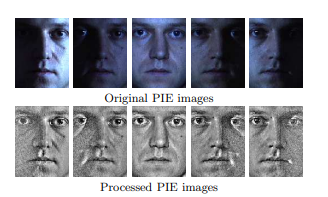
\includegraphics[width=0.5\textwidth]{beeld_voorbewerking.png}
    \caption{Beeld voorbewerking door het verwijderen van verschillende lichtinvallen. Bron: An Image Preprocessing Algorithm for Illumination Invariant Face Recognition \autocite{RalphBrajovic}}
\end{figure}


\subsection{Haar-achtige kenmerkdetectie}
Om het gezicht en de ogen te kunnen waarnemen, wordt er gebruik gemaakt van Haar-achtige kenmerkdetectie. Het meest gebruikte is AdaBoost vanwege zijn snelheid en nauwkeurigheid \autocite{Viola2004}.

Deze kenmerkdetectie houdt rekening met aangrenzende rechthoeken binnen een specifiek gebied in een bewegend detectievenster. Een afbeeldingsgebied kan omschreven worden als een combinatie van verschillende Haar-achtige kenmerken \autocite{Jibo2013}. Het aantal en types kunnen dan weer aangezien worden als verschillende objecten. De cumulatieve som van intensiteit vanaf de oorsprong wordt gedefinieerd als \begin{equation*}S_{i,j} = \sum_{x=0}^{i} \sum_{y=0}^{j} I(i, j)\end{equation*} Hierbij staat \( I_\text{(i,j)} \) voor de intensiteit op locatie (i,j), en \( S_\text{(i,j)} \) voor de cumulatieve som van intensiteiten vanaf de oorsprong op locatie (i,j). De som van intensiteit van de rechthoek, gedefinieerd als twee punten \( (x_{\text{links}}, y_{\text{boven}}) \) en  \( (x_{\text{rechts}}, y_{\text{onder}}) \), kan berekend worden volgens deze formule, die de berekening versnelt \begin{equation*}
    S_{\text{acc}}(x_{\text{rechts}}, y_{\text{onder}}) - S_{\text{acc}}(x_{\text{links}}, y_{\text{onder}}) - S_{\text{acc}}(x_{\text{rechts}}, y_{\text{boven}}) + S_{\text{acc}}(x_{\text{links}}, y_{\text{boven}})
\end{equation*}
\begin{itemize}
    \item \( S_{\text{acc}}(x_{\text{rechts}}, y_{\text{onder}}) \): Dit is de cumulatieve som van de intensiteiten tot het punt \( (x_{\text{rechts}}, y_{\text{onder}}) \). Het omvat alle pixelintensiteiten binnen en inclusief de rechthoek, vanaf de linkerbovenhoek tot de rechteronderhoek.
    \item \( S_{\text{acc}}(x_{\text{links}}, y_{\text{onder}}) \): Dit is de cumulatieve som van de intensiteiten tot het punt \( (x_{\text{links}}, y_{\text{onder}}) \). Het omvat alle pixelintensiteiten binnen en inclusief de rechthoek, vanaf de linkerbovenhoek tot de linkerbenedenhoek.
    \item \( S_{\text{acc}}(x_{\text{rechts}}, y_{\text{boven}}) \): Dit is de cumulatieve som van de intensiteiten tot het punt \( (x_{\text{rechts}}, y_{\text{boven}}) \). Het omvat alle pixelintensiteiten binnen en inclusief de rechthoek, vanaf de linkerbovenhoek tot de rechterbovenhoek.
    \item \( S_{\text{acc}}(x_{\text{links}}, y_{\text{boven}}) \): Dit is de cumulatieve som van de intensiteiten tot het punt \( (x_{\text{links}}, y_{\text{boven}}) \). Het omvat alle pixelintensiteiten binnen en inclusief de rechthoek, vanaf de linkerbovenhoek tot de linkerbovenhoek.
\end{itemize}


\subsection{Gezichtsdetectie}
Het gezicht wordt gedetecteerd door de Haar-achtige kenmerkdetectie \autocite{Viola2004}. Het zwaartepunt van het gezicht wordt berekend en vervolgens gebruikt om de knik- en rotatiebewegingen te meten van het gezicht. Een knikbeweging wordt gezien als de verticale beweging van het zwaartepunt groter is dan de horizontale beweging. Een rotatiebeweging werkt andersom \autocite{Jibo2013}. Een snelheid van 100 pixels per seconde wordt gebruikt als een grenswaarde voor de hoofdbewegingen in zowel horizontale als verticale richting.
\subsection{Detecteren van het oog}
Om het oog te kunnen detecteren zijn er verschillende algoritmes, deze zijn onder andere Hough-transformatie, patroonmatching, Principle Component Analysis (PCA) en het Adaboost algoritme. Het Adaboost algoritme maakt gebruikt van de Haar-achtige kenmerkdetectie \autocite{Viola2004}. Het ooggebied ligt horizontaal tussen 1/6 en 5/6 van het gezicht, terwijl het zich verticaal meestal tussen 1/4 en 1/2 bevindt. De breedte en hoogte van het gebied, dat dient om het oog te detecteren, wordt vastgesteld door de volgende formules: \begin{equation*}W_{gebied} = W_{gezicht} \times \frac{1}{4} \end{equation*} \begin{equation*}H_{gebied} = H_{gezicht} \times \frac{1}{3} \end{equation*}
\subsection{Knipperdetectie}
Een knipper wordt gedetecteerd doordat er een verandering is van zwarte pixels in het oog. Een open oog heeft een grotere pupil, dus meer zwarte pixels, dan een gesloten oog. Het oog wordt eerst omgezet naar een binair zwart-wit afbeelding. Vervolgens wordt de ratio van het aantal zwarte pixels berekend. Tenslotte dient deze ratio als een criterium om een knipper te detecteren.
\subsection{Oordelen van vermoeidheid}
Er zijn drie criteria die dienen om de vermoeidheid te oordelen. Deze zijn de frequentie van de knik- en rotatiebewegingen en PERCLOS (Percent Eye Closed). Een vermoeide bestuurder kan last hebben van frequente knikbewegingen en vaak knipperen. PERCLOS is een belangrijk en veelgebruikte indicator om vermoeidheid te detecteren. Het wordt gedefinieerd als het percentage tijd waarin dat de ogen gesloten zijn in een korte tijd (dit is vaak 30 seconden). Een oog wordt als gesloten beschouwd indien de zichtbare pupil kleiner is dan 30\% van zijn maximale opening. PERCLOS wordt als volgt berekend: \begin{equation*}PERCLOS = \frac{N}{30\times S}\end{equation*} waarin N staat voor het aantal knipperingen in de recentste 30 seconden, S is de bemonsteringsfrequentie.


\section{Artificiële Intelligentie}
Artificiële, beter gekend als kunstmatige, intelligentie is een manier voor machines om het `gedachteproces' van een mens na te bootsen. Hiermee zijn verschillende computerprogramma's in staat om te redeneren, conclusies te vormen en te antwoorden zoals bijna ieder hedendaags persoon kan. De meest bekende kunstmatige intelligentie, die bij zowaar niemand meer onbekend blijft, is ChatGPT. Dat in staat is om vragen te beantwoorden, meer uitleg geven over verschillende programmeertalen, wiskundige formules uit te leggen en op te lossen etc. Er is een continue ontwikkeling op dit vakgebied en wordt alsmaar meer geïmplementeerd in het dagelijks leven.

\subsection{Gezichtsdetectie}
AI heeft verschillende functionaliteiten. Zo is het in staat om het gezicht te detecteren van zowel foto's, video's en in real-time. Het kan echter wel zijn dat de nauwkeurigheid en de detectieratio aangetast worden. Dit wordt gedefinieerd als 'uitdagingen', enkele van deze zijn:
\begin{itemize}
    \item \textbf{Belichting}: Dit kan niet uniform zijn. Dat wil zeggen dat er enkele delen van het desbetreffende detectieframe meer of minder belicht zijn dan het andere deel.
    \item \textbf{Oriëntatie}: De richting hoe het gezicht gepositioneerd is.
    \item \textbf{Afstand}: De afstand van het gezicht ten opzichte van de camera.
    \item \textbf{Resolutie}: De resolutie van het beeld waarin het detecteren moet gebeuren.
    \item \textbf{Blokkeringen}: Één of meerdere objecten die tussenin de camera en het gezicht staan.
    \item \textbf{Complexe achtergronden}: Er zijn te veel objecten aanwezig in de achtergrond van het detectieframe.
\end{itemize}
Deze punten zorgen er elk voor dat er een extra uitdaging komt bij het detecteren van het gezicht, waardoor de nauwkeurigheid en het detectieratio verminderen \autocite{Kumar2019}. Binnenin het gebied van gezichtsdetectie, kunnen er verschillende detectietechnieken zijn. Deze technieken hebben elk een andere aanpak over hoe dat het gezicht wordt gedetecteerd.

\subsubsection{Active Shape Model}
Het doel van Active Shape Model (ASM) is om automatisch oriëntatiepunten te lokaliseren. Deze punten dienen om een vorm te definiëren. In het geval van het gezicht, focust het zich op de neus, ogen, mond, lippen en wenkbrauwen. ASM wordt getraind doordat er een statisch gezichtsmodel wordt gebouwd, met afbeeldingen waarop handmatig de oriëntatiepunten staan. ASM kan worden onderverdeeld in 3 groepen. Deze zijn Snakes, Point Distribution Model (PDM) en deformable templates.

\paragraph{Snakes}
Het eerste type maakt gebruikt van een generieke actieve omtrek, genaamd 'Snakes' \autocite{Kass1988}.
Snakes worden gebruikt om de grenzen van het hoofd te identificeren. Om deze taak uit te voeren, wordt er eerst een 'snake' geïnitialiseerd in de buurt van een hoofdgrens. Vervolgens gaat het opzoek naar nabijgelegen randen en neemt het stilaan de vorm van het hoofd aan. De evolutie hiervan wordt bereikt door het minimaliseren van een energiefunctie. Het wordt als volgt genoteerd:
\begin{equation*}
    E_{\text{snake}} = E_{\text{internal}} +  E_{\text{external}}
\end{equation*}
waarbij \(E_{\text{internal}} \) en \(E_{\text{external}} \) de interne en externe energiefuncties zijn.
De twee algemene overwegingen voor een snake te vormen zijn de selectie van energietermen en energie minimalisatie.
Elastische energie wordt hier gebruikt als interne energie \autocite{HJELMAS}. Dit varieert met de afstand tussen de controle punten van de snake. Hierdoor wordt er een omtrek verkregen dat in staat is om te vergroten of te verkleinen. Externe energie hangt dan echter weer af van de kenmerken van het beeld. Snakes hebben echter enkele nadelen. De omtrek komt vaak vast te zitten op valse beeldkenmerken en de snakes zijn niet geschikt voor het uittrekken van niet-convexe kenmerken.

\paragraph{Point Distribution Model}
Het Point Distribution Model (PDM) is onafhankelijk ontwikkeld van geautomatiseerde beeldanalyse en heeft statische modellen van vorm \autocite{HJELMAS}. Het idee achter PDM is dat men vormen kan voorstellen als vectoren. Nadien kunnen er standaard statische methodes op toegepast worden. De modellen leren toegestane situaties van vormpunten uit trainingsvoorbeelden en gebruiken vervolgens de hoofdcomponenten om het model op te bouwen. \textcite{Yuille1992} heeft het eerste parametrische statische vormmodel van beeldanalyse, dat gebaseerd is op de hoofdcomponenten van de oriëntatiepunten hun afstanden, gepresenteerd. Het PDM kan aanschouwd worden als het basismodel van Active Shape Model.

\paragraph{Deformable Templates}
%%=============================================================================
%% Methodologie
%%=============================================================================

\chapter{\IfLanguageName{dutch}{Methodologie}{Methodology}}%
\label{ch:methodologie}

%% TODO: In dit hoofstuk geef je een korte toelichting over hoe je te werk bent
%% gegaan. Verdeel je onderzoek in grote fasen, en licht in elke fase toe wat
%% de doelstelling was, welke deliverables daar uit gekomen zijn, en welke
%% onderzoeksmethoden je daarbij toegepast hebt. Verantwoord waarom je
%% op deze manier te werk gegaan bent.
%% 
%% Voorbeelden van zulke fasen zijn: literatuurstudie, opstellen van een
%% requirements-analyse, opstellen long-list (bij vergelijkende studie),
%% selectie van geschikte tools (bij vergelijkende studie, "short-list"),
%% opzetten testopstelling/PoC, uitvoeren testen en verzamelen
%% van resultaten, analyse van resultaten, ...
%%
%% !!!!! LET OP !!!!!
%%
%% Het is uitdrukkelijk NIET de bedoeling dat je het grootste deel van de corpus
%% van je bachelorproef in dit hoofstuk verwerkt! Dit hoofdstuk is eerder een
%% kort overzicht van je plan van aanpak.
%%
%% Maak voor elke fase (behalve het literatuuronderzoek) een NIEUW HOOFDSTUK aan
%% en geef het een gepaste titel.



\chapter{\IfLanguageName{dutch}{Proof-of-Concept}{Proof-of-Concept}}%
\label{ch:proof-of-concept}

\section{Introductie}
Als PoC wordt er een mobiele applicatie te ontwikkeld. Deze applicatie is in staat om het gezicht te detecteren en er bepaalde kenmerken uit te halen om vervolgens de vermoeidheid te berekenen. De reden waarom er voor een mobiele applicatie gekozen is is heel simpel. Tegenwoordig gebruikt iedereen wel een houdertje om zijn/haar gsm in te stoppen tijdens het rijden. Vaak is dit ook op de bestuurder gericht. Doordat dan onrechtstreeks de camera vaak op de bestuurder gericht staat, kan de applicatie vervolgens het gezicht detecteren en zo de conclusie er uit halen of hij al dan niet vermoeid is. De applicatie maakt gebruik van MediaPipe zijn Face Landmark detectie en breidt zo uit op het uitvoeren van formules voor het berekenen van Eye Aspect Ratio en PERCLOS.

\section{Doelstellingen}
Het belangrijkste doel van deze applicatie is, om door vermoeidheid te detecteren, het voorkomen van het gevaar in de verkeersveiligheid. Er gebeuren dagelijks wel wat ongevallen, zowel overdag als 's nachts. Één van de oorzaken voor ongevallen is dat de reactietijd van de bestuurder vaak te traag is door vermoeidheid. Uiteraard spelen er nog andere factoren een grote rol, maar de grootste oorzaak van nachtelijke ongevallen is toch wel vaak de vermoeidheid. Deze PoC zal er proberen voor zorgen dat dit zo snel mogelijk gedetecteerd kan worden en de bestuurder kan 'wakker' maken, zodat hij/zij zelf kan inschatten of ze beter zouden slapen dan verder rijden.

\section{Technologieën}
\subsection{Kotlin}
De applicatie wordt ontwikkeld in Kotlin. Sinds de Google I/O conferentie is er aangekondigd dat Android development Kotlin-first is. Dit houdt in dat dit gezien wordt als de primaire programmeertaal om een Android applicatie te ontwikkelen. Het biedt namelijk veel voordelen. Enkele van deze voordelen zijn:
\begin{itemize}
    \item \textbf{Minder code met een grotere leesbaarheid}: Je hoeft minder tijd te besteden aan het schrijven van code en is vaak sneller te begrijpen.
    \item \textbf{Minder veelvoorkomende fouten}: Applicaties die gebouwd zijn met Kotlin hebben, volgens de interne gegevens van Google, 20\% minder kans om vast te lopen.
    \item \textbf{Kotlin wordt ondersteunt in Jetpack libraries}: De aanbevolen moderne toolkit om een native UI in Kotlin te bouwen is Jetpack Compose. KTX-extenties voegen ook taalfunctionaliteiten van Kotlin toe. Deze zijn coroutines, extension functions, lambdas en genoemde parameters aan andere Android libraries.
    \item \textbf{Ondersteuning voor multiplatform development}: Kotlin Multiplatform zorgt ervoor dat de development niet enkel voor Android gebruikers is, maar ook voor iOS, backend en webapplicaties.
\end{itemize}

\subsection{MediaPipe}
Om het gezicht te kunnen detecteren heb ik gekozen om MediaPipe Solutions te gebruiken. Dit biedt een variatie van verschillende libraries en tools om snel en eenvoudig kunstmatige intelligentie (AI) en machine learning (ML) technieken kunt toepassen in je applicaties. Solutions maakt deel uit van het open source project MediaPipe, dit houdt in dat je de oplossingen makkelijk kunt aanpassen aan je behoeftes en je ze kan gebruiken op meerdere platformen.
\subsubsection{Face Detection}
Ik had er eerst voor gekozen om MediaPipe zijn Face Detection solution te gebruiken. Dit zette mij in staat om het gezicht te kunnen detecteren en er vervolgens een vierkant rond te zetten. Nadien kon je de punten van interesse op zetten. Dit wil zeggen dat je kon aanduiden via een stip waar de ogen, mond, neus en oren zich bevonden. Al snel kwam ik er achter dat MediaPipe over een ander soort solution beschikte die mij meer kon helpen.
\subsubsection{Face Landmark Detection}
Deze solution zorgde ervoor dat ik een betere representatie had van het gezicht. Dit was in staat om zowel het gezicht te detecteren als de expressie. Het maakt gebruik van ML modellen die kunnen werken met zowel enkele afbeeldingen als een stroom van afbeeldingen. De output van deze solution was een virtuele avatar. Het maakte drie-dimensionele landmark punten op het gezicht. Bovendien gaf het ook een score van welke expressie het detecteert. 

\section{Implementatie}
De implementatie van de Proof of Concept (PoC) is onderverdeeld in enkele stappen. Elke stap draagt bij aan het geheel van de applicatie.

\subsection{Algemeen}
\subsubsection{Navigatie}
Eerst en vooral wordt er een navigatie voorzien. Hierin bevinden zich twee fragments. Zo heb je een \emph{PermissionFragment} en \emph{CameraFragment}. Dit gebeurt zodat de overschakeling van het ene fragment naar het andere fragment soepeler verloopt.
\begin{lstlisting}[language=Kotlin, caption=nav\_graph.xml]
    <navigation xmlns:android="http://schemas.android.com/apk/res/android"
        xmlns:app="http://schemas.android.com/apk/res-auto"
        android:id="@+id/nav_graph"
        app:startDestination="@id/permissions_fragment"> 
    </navigation>
\end{lstlisting}
\begin{itemize}
    \item \textbf{xmlns:android}: De XML-namespace voor standaard Android-attributen
    \item \textbf{xmlns:app}: De XML-namespace voor aangepaste attributen.
    \item \textbf{xmlns:id}: De unieke ID voor de layout.
    \item \textbf{xmlns:starDestination}: Het fragment dat als eerst moet worden weergegeven als de applicatie is opgestart.
\end{itemize}

\subsubsection{CoordinatorLayout}
Bepaalde fragments bestaan uit verschillende views. Deze views worden samen in een  \emph{CoordinatorLayout} gezet. Dit maakt coördinatie tussen de verschillende views mogelijk. Zo kun je meerdere views in één fragment hebben.
\begin{lstlisting}[language=Kotlin, caption=CoordinatorLayout]
    <androidx.coordinatorlayout.widget.CoordinatorLayout
        xmlns:android="http://schemas.android.com/apk/res/android"
        xmlns:app="http://schemas.android.com/apk/res-auto"
        android:id="@+id/camera_container"
        android:layout_width="match_parent"
        android:layout_height="match_parent">
    </androidx.coordinatorlayout.widget.CoordinatorLayout>
\end{lstlisting}

\begin{itemize}
    \item \textbf{xmlns:android}: De XML-namespace voor standaard Android-attributen
    \item \textbf{xmlns:app}: De XML-namespace voor aangepaste attributen.
    \item \textbf{xmlns:id}: De unieke ID voor de layout.
    \item \textbf{xmlns:layout\_width}: Breedte van de layout. Deze staat ingesteld op \emph{match\_parent} om de volledige breedte van het scherm te gebruiken.
    \item \textbf{xmlns:layout\_height}: Hoogte van de layout. Deze staat ingesteld op \emph{match\_parent} om de volledige hoogte van het scherm te gebruiken.
\end{itemize}


\subsection{Camera}
De implementatie van de PoC begint met het initialiseren van de camera. De camera is een cruciaal onderdeel van de applicatie omdat deze de input levert voor de verdere verwerking en analyse. Zonder een goed werkende camera kan de applicatie niet functioneren zoals bedoeld.

Voor deze applicatie maak ik gebruik van de CameraX bibiliotheek, die een eenvoudige en consistente API biedt voor cameratoegang en -beheer voor verschillende Android apparaten. In deze sectie toon ik even aan hoe het gebruik van de camera tot stand is gekomen.

\subsubsection{PermissionFragment}
Uiteraard heb ik toestemming nodig van de gebruiker om de camera te mogen gebruiken. Hiervoor is er een \emph{PermissionFragment} voorzien. Dit toont zich ook in de navigatie. Dit ziet er als volgt uit:
\begin{lstlisting}[language=Kotlin, caption=PermissionFragment]
    <fragment
    android:id="@+id/permissions_fragment"
    android:name="com.example.bach_poc.fragments.PermissionsFragment"
    android:label="PermissionsFragment">
    
    <action
    android:id="@+id/action_permissions_to_camera"
    app:destination="@id/camera_fragment"
    app:popUpTo="@id/permissions_fragment"
    app:popUpToInclusive="true" />
    </fragment>
\end{lstlisting}
De belangrijkste attributen van de fragment tag zijn \emph{android:id} en \emph{android:name}. Het eerste attribuut is de unieke ID van het fragment binnenin de navigatie. Deze ID wordt dus ook gebruikt om naar dit fragment te verwijzen bij navigatieacties. Het tweede attribuut is de naam van de klasse van het fragment. In dit geval zal er de klasse \emph{PermissionsFragment} gebruikt worden. Binnen in de action tag zijn er nog andere attributen. Zo heb je \emph{app:destination}, wat de bestemming van de navigatieactie is, \emph{app:popUpTo}, wat specificeert tot welk punt de backstack gewist zal worden en \emph{app:popUpToInclusive}, wat er voor zorgt dat 'permissions\_fragment' ook uit de backstack gewist zal worden.

Nu zal er wat uitleg gegeven worden over wat er precies in de klasse \emph{PermissionsFragment.kt} zit. Om aan te tonen dat deze klasse een fragment is, zal het dan ook overerven van \emph{Fragment}. Deze heeft een methode \emph{onCreate} die wordt opgeroepen om de gebruikersinterface te creëren.
\begin{lstlisting}[language=Kotlin,caption=override fun onCreate(savedInstanceState: Bundle?) in PermissionsFragment.kt, label={lst:onCreatePermissions}]
    override fun onCreate(savedInstanceState: Bundle?) {
        super.onCreate(savedInstanceState)
        when {
            ContextCompat.checkSelfPermission(
            requireContext(),
            Manifest.permission.CAMERA
            ) ==
            PackageManager.PERMISSION_GRANTED -> {
                navigateToCamera()
            }
            else -> {
                requestPermissionLauncher.launch(Manifest.permission.CAMERA)
            }
        }
    }
\end{lstlisting}
Zodra de fragment gemaakt wordt, wordt de basisimplementatie van \emph{Fragment} uitgevoerd. Vervolgens wordt er gecontroleerd of de benodigde permissie verleend is. Dit gebeurt in de \emph{when} conditie. Die gaat de permissie voor de camera ophalen en controleren of hij al dan niet verleend is, dit gebeurt door de conditie in de accolades na \emph{when}. Dit haalt de context van het fragment op inclusief \emph{Manifest.permission.CAMERA}, wat de constante is die de camera-permissie vertegenwoordigt. Vervolgens kijkt hij of de permissie wel degelijk toegelaten is (\emph{PackageManager.PERMISSION\_GRANTED}). Indien de permissie niet is toegelaten, zal hij de popup lanceren die vraagt naar de toestemming.

\begin{lstlisting}[language=Kotlin, caption=requestPermissionLauncher in PermissionsFragment.kt, label={lst:requestPermissionLauncher}]
    private val requestPermissionLauncher =
    registerForActivityResult(ActivityResultContracts.RequestPermission()) { 
        isGranted: Boolean ->
            if (isGranted) {
                Toast.makeText(
                context,
                "Permission request granted",
                Toast.LENGTH_LONG
                ).show()
                navigateToCamera()
            } else {
                Toast.makeText(
                context,
                "Permission request denied",
                Toast.LENGTH_LONG
                ).show()
            }
        }
\end{lstlisting}
Hierbij wordt er een \emph{ActivityResultLauncher} gelanceerd. Die zal de permissieaanvraag uitvoeren. De callbackfunctie \emph{isGranted} zal de boolean opslaan en zal vervolgens een passend bericht aan tonen als de aanvraag geaccepteerd of afgewezen is.

\begin{lstlisting}[language=Kotlin, caption=navigateToCamera() in PermissionsFragment.kt]
    private fun navigateToCamera() {
        lifecycleScope.launch {
            lifecycle.repeatOnLifecycle(Lifecycle.State.STARTED) {
                Navigation.findNavController(
                requireActivity(),
                R.id.fragment_container
                )
                .navigate(R.id.camera_fragment)
            }
        }
    }
    
\end{lstlisting}
Deze functie wordt uitgevoerd indien de permissie van de camera wel toegelaten is. Er wordt een nieuwe coroutine gestart door \emph{lifecycleScope.launch}. Een coroutine is gekoppeld aan de levenscyclus van een fragment, in dit geval van \emph{PermissionsFragment.kt}. Dit wil zeggen dat het dus geannuleerd wordt indien het fragment of de activiteit 'vernietigd' wordt. Door de regel \emph{lifecycle.repeatOnLifecycle(Lifecycle.State.STARTED)} zal de code binnenin dat codeblock enkel uitgevoerd worden wanneer het fragment in de toestand 'STARTED' is. Vervolgens wordt er genavigeerd naar het fragment met id \emph{camera\_fragment} vanuit de huidige fragment.

\begin{lstlisting}[language=Kotlin, caption=companion object van PermissionsFragment.kt, label={lst:companionPermssion}]
private val PERMISSIONS_REQUIRED = arrayOf(Manifest.permission.CAMERA)

companion object {
    fun hasPermissions(context: Context) =
    PERMISSIONS_REQUIRED.all {
        ContextCompat.checkSelfPermission(
        context,
        it
        ) == PackageManager.PERMISSION_GRANTED
    }
}
\end{lstlisting}
Dit is het \emph{companion object} van \emph{PermissionsFragment}. Deze functie is gekoppeld aan de definitie van de klasse, wat dus wilt zeggen is dat het de functie zal uitvoeren bij het instantiëren. In dit geval return de functie een \emph{boolean} om te kijken of de permissies die in \emph{PERMISSIONS\_REQUIRED} staan zijn toegelaten of niet.

\subsubsection{CameraFragment}
Net zoals \emph{PermissionFragment} erft \emph{CameraFragment} ook over van \emph{Fragment}, maar ook van \emph{FaceLandmarkerHelper.LandmarkListener}, waar nog verdere uitleg over zal gegeven worden.
In tegenstelling tot de \emph{PermissionsFragment} beschikt deze fragment over enkele variabelen die in het geheel van de klasse worden gebruikt. Deze variabelen zullen vermeld worden bij de methodes die ze gebruiken.

\begin{lstlisting}[language=Kotlin, caption=onCreateView in CameraFragment.kt, label={lst:onCreateViewCameraFragment}]
    private var _fragmentCameraBinding: FragmentCameraBinding? = null
    private val fragmentCameraBinding get() = _fragmentCameraBinding!!

    override fun onCreateView(
        inflater: LayoutInflater,
        container: ViewGroup?,
        savedInstanceState: Bundle?): View?
        {
            _fragmentCameraBinding = FragmentCameraBinding
                                .inflate(inflater,container,false)
    
            return fragmentCameraBinding.root
        }
\end{lstlisting}
Deze methode wordt uitgevoerd terwijl de view wordt aangemaakt. De variabele \emph{\_fragmentCameraBinding} is een gegenereerde klasse dat overeenkomt met de layout file van het fragment (\emph{fragment\_camera.xml}). Nadien wordt de variabele \emph{fragmentCameraBinding} gebruikt als een \emph{get()} functie om het fragment effectief te verkrijgen. De methode \emph{onCreateView} gaat de view van de camera maken. Dit doet hij door het fragment 'op te blazen' met de view, wat dus wilt zeggen dat de view in de layout wordt gestopt. Daarna wordt de top-level view gereturned (\emph{fragmentCameraBinding.root}).

\begin{lstlisting}[language=Kotlin, caption=onViewCreated in CameraFragment.kt, label={lst:onViewCreatedCameraFragment}]
    private lateinit var backgroundExecutor: ExecutorService
    
     private val faceBlendshapesResultAdapter by lazy {
        FaceBlendshapesResultAdapter()
    }
    
    
    @SuppressLint("MissingPermission")
    override fun onViewCreated(view: View, savedInstanceState: Bundle?) {
        super.onViewCreated(view, savedInstanceState)
        
        with(fragmentCameraBinding.recyclerviewResults) {
            layoutManager = LinearLayoutManager(requireContext())
            adapter = faceBlendshapesResultAdapter
        }
        
        backgroundExecutor = Executors.newSingleThreadExecutor()
        
        fragmentCameraBinding.viewFinder.post {
            setUpCamera()
        }
        
        backgroundExecutor.execute {
            faceLandmarkerHelper = FaceLandmarkerHelper(
            context = requireContext(),
            minFaceDetectionConfidence = 0.5F,
            minFacePresenceConfidence = 0.5F,
            minFaceTrackingConfidence = 0.5F,
            maxNumFaces = 1,
            currentDelegate = 0,
            faceLandmarkerHelperListener = this
            )
        }
    }
\end{lstlisting}
Deze methode maakt gebruik van een \emph{ExecutorService}. Dit is een extensie van \emph{Executor}. Deze service zorgt er voor dat er asynchrone taken uitgevoerd kunnen worden. De \emph{@SuppressLint(`MissingPermission`)} is een annotatie dat de lint-waarschuwing onderdrukt voor ontbrekende toestemmingen, deze zijn namelijk al behandeld in \emph{PermissionFragment}. Nadat de view gemaakt is, wordt dit allemaal uitgevoerd.

De \emph{RecyclerView} van de layout wordt eerst opgehaald in het \emph{with} blok, dit zal later nog uitgelegd worden. De \emph{layoutManager} is hetgeen wat de layout zal beheren, de adapter wordt ingesteld als een hulpklasse van \emph{FaceBlendshapesResultAdapter}, dit is verantwoordelijk voor het weergeven van de resultaten van de gezichtsanalyse en zal nog verder uitgelegd worden.

Nadien wordt er een \emph{backgroundExecutor} gemaakt. Dit is een thread executor dat verdere taken op de achtergrond zal uitvoeren. Na al deze elementen geïnitialiseerd zijn zal de camera zich klaarmaken voor gebruik. Dit gebeurt echter enkel als de view gemaakt is en de \emph{viewFinder} beschikbaar is. Tenslotte zal de \emph{backgroundExecutor} een \emph{FaceLandmarkerHelper} maken op de achtergrond. De parameters van deze klasse worden later besproken.

\begin{lstlisting}[language=Kotlin, caption=setUpCamera in CameraFragment.kt, label={lst:setUpCamera}]
    private var cameraProvider: ProcessCameraProvider? = null
    
    private fun setUpCamera() {
        val cameraProviderFuture = ProcessCameraProvider
                                        .getInstance(requireContext())
        cameraProviderFuture.addListener(
        {
            cameraProvider = cameraProviderFuture.get()
            
            bindCameraUseCases()
        },
        ContextCompat.getMainExecutor(requireContext())
        )
    }
\end{lstlisting}
Hier wordt de camera klaargemaakt voor gebruik. Deze methode instantieert de variabele \emph{cameraProvider}. Dit is een singleton wat gebruikt wordt om de levenscyclus van de camera aan te koppelen. Binnenin de functie wordt de instantie van de huidige context van de applicatie gedeclareerd aan een nieuwe variabele. Vervolgens wordt er een \emph{listener} toegevoegd aan de instantie.

De code binnenin de accolades van de \emph{addListener} wordt uitgevoerd zodra de algemene executor van de context wordt opgehaald in \emph{ContextCompat.getMainExecutor(requireContext())}. In die blok van code wordt de \emph{cameraProvider} gedeclareerd en worden de usecases van de camera ingesteld (\emph{bindCameraUseCases}).

\begin{lstlisting}[language=Kotlin, caption=bindCameraUseCases in CameraFragment.kt, label{lst:bindCameraUseCases}]
    private var preview: Preview? = null
    private var imageAnalyzer: ImageAnalysis? = null
    private var camera: Camera? = null
    private fun bindCameraUseCases() {
     
        val cameraProvider = cameraProvider?:
                            throw IllegalStateException("Camera initialization failed.")
        
     
        val cameraSelector = CameraSelector.Builder()
        .requireLensFacing(CameraSelector.LENS_FACING_FRONT).build()
        
        val screenSize = Size(640, 480)
        val resolutionSelector = ResolutionSelector.Builder()
                            .setResolutionStrategy(ResolutionStrategy(screenSize,
                            ResolutionStrategy.FALLBACK_RULE_NONE)).build()
        
        preview = Preview.Builder()
        .setResolutionSelector(resolutionSelector)
        .build()
        
        
        imageAnalyzer = ImageAnalysis.Builder()
        .setResolutionSelector(resolutionSelector)
        .setBackpressureStrategy(ImageAnalysis.STRATEGY_KEEP_ONLY_LATEST)
        .setOutputImageFormat(OUTPUT_IMAGE_FORMAT_RGBA_8888)
        .build()
        .also {
            it.setAnalyzer(backgroundExecutor) { image ->
                detectFace(image)
            }
        }
        
        
        cameraProvider.unbindAll()
        
        try {
            camera = cameraProvider.bindToLifecycle(
            this,
            cameraSelector,
            preview,
            imageAnalyzer
            )
            
            preview?.setSurfaceProvider(fragmentCameraBinding
                                            .viewFinder.surfaceProvider)
        } catch (exc: Exception) {
            Log.e(TAG, "Use case binding failed", exc)
        }
    }
\end{lstlisting} 
Deze methode heeft nood aan wat extra variabelen. We maken gebruik van \emph{Camera}, \emph{Preview} en \emph{ImageAnalyzer}. Eerst en vooral wordt er gekeken of de \emph{cameraProvider} al dan niet bestaat. Indien hij niet bestaat, zal er een \emph{IllegalStateException} gegooid worden. 

Vervolgens wordt de richting van de camera ingesteld. Dit gebeurt door \emph{CameraSelector.Builder().requireLensFacing(CameraSelector.LENS\_FACING\_FRONT).build()}. Dit roept de interface van de camera op en laat zo weten dat we behoefte hebben aan het gebruik van de selfie-camera.

Voor dat de preview van de camera gebuild wordt, zodat we ons zelf kunnen zien, is er nood aan het instellen van een \emph{ResolutionSelector}. Dit stelt de resolutie van de \emph{UseCase} in. De schermgrootte wordt ingesteld op 640x480 pixels en wordt vervolgens gebruikt om een \emph{ResolutionStrategy} in te stellen. Tenslotte kan zo de \emph{ResolutionSelector} van de \emph{UseCase} gebuild worden. 
 
Nadat we een resolutie hebben, kan de \emph{Preview} gemaakt worden. De \emph{Preview} zorgt er voor dat we de camera kunnen bekijken die gebruikt wordt, we kunnen onszelf dus zien. 

Nadien wordt er een \emph{ImageAnalyzer} gedeclareerd. Dit zorgt ervoor dat we het beeld kunnen analyseren dat wordt opgenomen. Deze analyzer gebruikt dezelfde instellingen voor de resolutie als die van de camera. Dit doe ik zodat het camerabeeld direct geanalyseerd kan worden en niet eerst nog omgezet moet worden naar eventueel een andere resolutie voor de analyse. De \emph{.setBackpressureStrategy} wordt ingesteld op \emph{STRATEGY\_KEEP\_ONLY\_LATEST}. Dit wilt zeggen dat enkel de laatste \emph{image} wordt doorgestuurd naar de analyzer, de voorgaande worden dus gedropt. Dit is noodzakelijk doordat sommige frames sneller verstuurd worden dan dat ze geanalyseerd worden. De analyzer zal de images die hij moet analyseren ontvangen in \emph{RGBA\_8888} formaat. Het wordt dus verstuurd met een Rood, Groen, Blauw en Alpha waarde. De 8888 staat voor het aantal bits dat gebruikt wordt om elke waarde te coderen. Dit is het standaardformaat. Tenslotte wordt de analyzer gebuild en zal er een analyzer voor de \emph{backgroundExecutor} ingesteld worden, die zal op de achtergrond het gezicht detecteren van de image.

Voordat er nieuwe use cases aan de \emph{cameraProvider} gebonden kunnen worden, moeten ze eerst ontbonden worden. Dit gebeurt door \emph{.unbindAll()}. Dit zorgt er voor dat, indien er andere fragments bestaan die ook bindingen hebben aan de provider, al de bindingen zich ontbinden.

Als laatste stap worden de 3 use cases: \emph{CameraSelector}, \emph{Preview} en \emph{ImageAnalysis} gebonden aan de levenscyclus van de cameraprovider en het oppervlak van de \emph{viewFinder} zich aan de preview binden. Indien dat niet lukt, zal er zich een error voordoen.

\begin{lstlisting}[language=Kotlin, caption=detectFace in CameraFragment.kt, label={lst:detectFace}]
    
    private fun detectFace(imageProxy: ImageProxy){
        faceLandmarkerHelper.detectLivestream(
        imageProxy = imageProxy
        )
    }
    
\end{lstlisting}
De methode \emph{detectFace} gaat het beeld van de \emph{ImageAnalyzer} nemen en gaat de methode \emph{detectLiveStream(ImageProxy imageProxi)} oproepen die in de \emph{FaceLandmarkerHelper} staat.

We zien dat \emph{CameraFragment} overerft van \emph{FaceLandMarkerHelper.Listener}. Dit is een interface die in \emph{FaceLandmarkerHelper} staat. Deze beschikt over 3 methodes: \emph{onError}, \emph{onEmpty} en \emph{onResults}.
\begin{lstlisting}[language=Kotlin, caption=onError in CameraFragment.kt, label={lst:onError}]
override fun onError(error: String, errorCode: Int) {
    activity?.runOnUiThread {
        Toast.makeText(requireContext(), error, Toast.LENGTH_SHORT).show()
        faceBlendshapesResultAdapter.updateResults(null)
        faceBlendshapesResultAdapter.notifyDataSetChanged()
    }
}
\end{lstlisting}
Dit zorgt ervoor dat de gebruiker op de hoogte wordt gebracht indien er zich een fout voordoet. Als er effectief een fout voorkomt, zullen de resultaten op \emph{null} worden ingesteld en wordt er aan \emph{faceBlendshapesResultdAdapter} gecommuniceerd dat de dataset veranderd is.

\begin{lstlisting}[language=Kotlin, caption=onEmpty in CameraFragment.kt, label={lst:onEmpty}]
    override fun onEmpty() {
        fragmentCameraBinding.overlay.clear()
        activity?.runOnUiThread {
            faceBlendshapesResultAdapter.updateResults(null)
            faceBlendshapesResultAdapter.notifyDataSetChanged()
        }
    }
\end{lstlisting}
Deze methode zal er voor zorgen dat de applicatie reageert als er geen gezicht wordt gedetecteerd. Hij wist ook de mogelijke visuele overlay en zal ook de resultaten op \emph{null} gezet worden.

\begin{lstlisting}[language=Kotlin, caption=onResults in CameraFragment.kt, label={lst:onResults}]
    override fun onResults(resultBundle: FaceLandmarkerHelper.ResultBundle) {
        activity?.runOnUiThread {
            if (_fragmentCameraBinding != null) {
                if (fragmentCameraBinding.recyclerviewResults
                                        .scrollState != SCROLL_STATE_DRAGGING)
                {
                    faceBlendshapesResultAdapter
                                    .updateResults(resultBundle.result)
                    faceBlendshapesResultAdapter.notifyDataSetChanged()
                }
                
                fragmentCameraBinding.overlay.setResults(
                resultBundle.result,
                resultBundle.inputImageHeight,
                resultBundle.inputImageWidth,
                )
                fragmentCameraBinding.overlay.invalidate()
            }
        }
    }
\end{lstlisting}
Deze methode zal de resultaten van de camera doorgeven aar \emph{faceBlendshapesResultAdapater} indien er niet gescrolled wordt op de applicatie. Vervolgens zullen de resultaten ook doorgegeven worden aan het overlay component. Dit component zal tonen waar het gezicht gedetecteerd is.

\subsection{Face Landmark Detectie}
Om het gezicht te kunnen detecteren en weer te geven aan de gebruiker, zijn er enkele hulpklassen gemaakt. Deze klassen zorgen ervoor dat het doorgegeven beeld gebruikt kan worden om daarop het gezicht te detecteren en nadien een visueel beeld kan returnen van de landmarks.

\subsubsection{FaceLandmarkerHelper}
Deze klasse zal het gezicht op het beeld detecteren. Dit kan gezien worden als de basis van de gezichtsdetectie. Nu zullen de methoden die gebruikt zijn in deze klasse uitgelegd worden. Voor dat we de verder duiken in deze klasse, zal er eerst wat informatie gegeven worden over het \emph{companion object} zodat we toegang hebben tot verschillende constanten bij het aanmaken van deze klasse.

\begin{lstlisting}[language=Kotlin, caption=companion object van FaceLandmarkerHelper.kt, label={lst:companionFaceLandmarkerHelper}]
    companion object {
        const val TAG = "FaceLandmarkerHelper"
        private const val MP_FACE_LANDMARKER_TASK = "face_landmarker.task"
        
        const val DELEGATE_CPU = 0
        const val DELEGATE_GPU = 1
        const val DEFAULT_FACE_DETECTION_CONFIDENCE = 0.5F
        const val DEFAULT_FACE_TRACKING_CONFIDENCE = 0.5F
        const val DEFAULT_FACE_PRESENCE_CONFIDENCE = 0.5F
        const val DEFAULT_NUM_FACES = 1
        const val OTHER_ERROR = 0
        const val GPU_ERROR = 1
        
    }
\end{lstlisting}
De constante \emph{TAG} wordt vooral gebruikt bij het loggen. Indien er zich dan een fout voordoet, kan er in de logs gekeken worden in welke klasse deze error zich voordoet. \emph{MP\_FACE\_LANDMARKER\_TASK} is de constante dat een relatie legt aan de \emph{task} die het detecteren zal volbrengen. Deze taak is in de \emph{assets} folder gezet. De overige constanten die ingesteld staan als parameters om de taak aan te passen.

\begin{lstlisting}[language=Kotlin, caption=interface LandmarkListener, label={lst:interfaceLandmarkListener}]
     interface LandmarkListener {
        fun onError(error: String, errorCode: Int = OTHER_ERROR)
        fun onResults(resultBundle: ResultBundle)
        fun onEmpty() {}
    }
\end{lstlisting}
Dit is de interface \emph{LandmarkListener}. Doordat we \emph{RunningMode.LIVE\_STREAM} gebruiken, hebben we nood aan deze interface. Deze methodes zijn uitgeschreven in \emph{CameraFragment}. Dit houdt dus in dat dit eigenlijk een \emph{LandmarkListener} is en dus de resultaten asynchroon zal ontvangen.


\begin{lstlisting}[language=Kotlin, caption=init() en setupFaceLandmarker() in FaceLandmarkerHelper.kt, label={lst:setupFaceLandmarker}]
    init {
        setupFaceLandmarker()
    }
    
    private var faceLandmarker: FaceLandmarker? = null
    
    fun setupFaceLandmarker() {
        val baseOptionBuilder = BaseOptions.builder()
        
        when (currentDelegate) {
            DELEGATE_CPU -> {
                baseOptionBuilder.setDelegate(Delegate.CPU)
            }
            DELEGATE_GPU -> {
                baseOptionBuilder.setDelegate(Delegate.GPU)
            }
        }
        
        baseOptionBuilder.setModelAssetPath(MP_FACE_LANDMARKER_TASK)
        
        if (faceLandmarkerHelperListener == null) {
            throw IllegalStateException(
                    "faceLandmarkerHelperListener must be set when runningMode is LIVE_STREAM")
        }
        
        try {
            val baseOptions = baseOptionBuilder.build()
            val optionsBuilder =
            FaceLandmarker.FaceLandmarkerOptions.builder()
            .setBaseOptions(baseOptions)
            .setMinFaceDetectionConfidence(minFaceDetectionConfidence)
            .setMinTrackingConfidence(minFaceTrackingConfidence)
            .setMinFacePresenceConfidence(minFacePresenceConfidence)
            .setNumFaces(maxNumFaces)
            .setOutputFaceBlendshapes(true)
            .setRunningMode(RunningMode.LIVE_STREAM)
            .setResultListener(this::returnLivestreamResult)
            .setErrorListener(this::returnLivestreamError)
            
            val options = optionsBuilder.build()
            faceLandmarker = FaceLandmarker.createFromOptions(context,options)
        } catch (e: IllegalStateException) {
            faceLandmarkerHelperListener?.onError(
            "Face Landmarker failed to initialize, See error logs for details"
            )
            Log.e(TAG, "MediaPipe failed to load the task with error" + e.message)
        }
        catch (e: RuntimeException) {
            faceLandmarkerHelperListener?.onError(
            "Face Landmarker failed to initialize. See error logs for " +
            "details", GPU_ERROR
            )
            Log.e(TAG, "Face Landmarker failed to load model with error: " + 
                                                                        e.message)
        }
    }
\end{lstlisting}

De klasse wordt geïnitialiseerd door een \emph{init()} methode. In die methode wordt \emph{setupFaceLandmarker} opgeroepen. Het grote beeld van deze methode is het gereedmaken van het gebruik van de \emph{Face Landmark detectie}.

Eerst en vooral wordt er een \emph{BaseOptions} ingesteld. Die opties vormen de basis van de taak. Het eerste \emph{if} statement gaat selecteren wat de taak gaat uitvoeren. Dat kan zowel de CPU als de GPU zijn, afhankelijk van hoe het is ingesteld. In het geval van deze Proof of Concept is het de CPU. Doordat onze applicatie niet zo krachtig is, heeft het geen impact op de performance, je zou dus evengoed de GPU kunnen kiezen. De \emph{currentDelegate} wordt meegegeven als parameter en staat ingesteld op \textbf{\emph{var currentDelegate: Int = DELEGATE\_CPU}}. Er kan dus een andere delegate meegegeven worden indien dat gewenst is, anders zal de CPU gebruikt worden.

Vervolgens wordt het pad van de taak ingesteld. Dit is de constante
\emph{MP\_FACE\_LANDMARKER\_TASK} die we in het \emph{companion object} gedeclareerd hebben. Zo weet de \emph{BaseOptions} welke taak hij moet uitvoeren, in dit geval \emph{face\_landmarker.task}.

Het \emph{if} statement nadat het \emph{assetPath} is ingesteld, kijkt of er wel een \emph{faceLandmarkerHelperListener} is. Ook dit is een parameter van deze klasse \textbf{\emph{var faceLandmarkerHelperListener: LandmarkListener? = null}}. Een \emph{LandmarkListener} is noodzakelijk wanneer de \emph{RUNNING.MODE} wordt ingesteld op livestream. Zo krijgen we een continue detectie en analyse. Eerder gezien in de \emph{onViewCreated} wordt \emph{CameraFragment} meegegeven als \emph{LandmarkListener}. Zo weet de taak of er nieuwe beelden binnenkomen, wat in dit geval constant is.

Tenslotte wordt er een \emph{try catch} uitgevoerd. In het try gedeelte van de code wordt eerst en vooral de \emph{baseOptions} gebuild. Nadien wordt de \emph{optionsBuilder} samengesteld. Dit gaat de \emph{FaceLandmarker} builden. Daar horen enkele zaken bij:
\begin{itemize}
    \item \textbf{setBaseOptions}: De basisopties van de taak. In dit geval de delegate dat gebruikt wordt.
    \item \textbf{setMinFaceDetectionConfidence(minFaceDetectionConfidence)}: De minimum zelfzekerheid score voor het gezicht dat moet voldoen om het detecteren een succes te noemen. Staat ingesteld op 0.5.
    \item \textbf{setMinTrackingConfidence(minFaceTrackingConfidence)}: De minimum zelfzekerheid score voor het traceren van het gezicht. Staat ingesteld op 0.5.
    \item \textbf{setMinFacePrsenceConfidence(minFacePresenseConfidence)}: De minimum zelfzekerheid score van het gezicht dat aanwezig is. Staat ingesteld op 0.5.
    \item \textbf{setNumFaces(maxNumFaces)}: Het maximum aantal gezichten dat gedetecteerd kan worden. Staat ingesteld op 1.
    \item \textbf{setOutputFaceBlendshapes(true)}: Dit zorgt ervoor dat het resultaat gebruikt kan worden voor het renderen van een 3D model.
    \item \textbf{setRunningMode(RunningMode.LIVE\_STREAM)}: RunningMode van de taak. Sinds het \emph{LIVE\_STREAM} is, moet er een \emph{resultListener} worden meegegeven om de resultaten asynchroon te ontvangen.
    \item \textbf{setResultListener(this::returnLiveStreamResult)}: Zorgt ervoor dat de resultaten asynchroon ontvangen worden. Kan enkel gebruikt worden als de RunningMode ingesteld staat op \emph{LIVE\_STREAM}
    \item \textbf{setErrorListener(this::returnLiveStreamError)}: Optionele \emph{listener} die errors gaat afhandelen.
\end{itemize}
Al de parameters die hierboven zijn gebruikt, staan in het \emph{companion object}. Nadat de taak succesvol geconfigureerd is, zal hij gebouwd worden. Indien er ergens iets mis loopt in het \emph{try} blok, zijn er \emph{catch} blokken voorzien om de errors te melden.

\begin{lstlisting}[language=Kotlin, caption=returnLiveStreamResult in FaceLandmarkerHelper.kt, label={lst:returnLiveStreamResult}]
    private fun returnLivestreamResult(
    faceLandmarkerResult: FaceLandmarkerResult,
    mpImage: MPImage
    ) {
        if (faceLandmarkerResult.faceLandmarks().size > 0) {
            val finishTimeMs = SystemClock.uptimeMillis()
            val inferenceTime = finishTimeMs - faceLandmarkerResult.timestampMs()
            
            faceLandmarkerHelperListener?.onResults(
            ResultBundle(
            faceLandmarkerResult,
            inferenceTime,
            mpImage.height,
            mpImage.width
            )
            )
        }
        else {
            faceLandmarkerHelperListener?.onEmpty()
        }
    }
    
    data class ResultBundle(
        val result: FaceLandmarkerResult,
        val inferenceTime: Long,
        val inputImageHeight: Int,
        val inputImageWidth: Int,
    )
\end{lstlisting}
Deze methode zal het resultaat teruggeven van de detectie. Deze functie heeft als parameters \emph{FaceLandmarkerResult} en \emph{MPImage}. Het doel van deze functie is het controleren of er daadwerkelijk gezichten gedetecteerd zijn of niet. Indien dit het geval is, zal er berekend worden hoelang het geduurd heeft tot de resultaten. Dit gebeurt door \emph{inferenceTime}. Het is de tijd sinds de applicatie is opgestart - de tijd dat het geduurd heeft om een gezicht te detecteren. Tenslotte wordt er een \emph{ResultBundle} gemaakt. Daarin zit het resultaat, de tijd en de hoogte en breedte van de camerabeelden. Als er geen gezichten gedetecteerd zijn, zal de \emph{onEmpty()} functie opgeroepen worden.

\begin{lstlisting}[language=Kotlin, caption=returnLiveStreamError in FaceLandmarkerHelper.kt, label={lst:returnLivestreamError}]
    private fun returnLivestreamError(runtimeException: RuntimeException) {
        faceLandmarkerHelperListener?.onError(
        runtimeException.message ?: "An unknown error has occurred"
        )
    }
\end{lstlisting}
Dit is de functie die een error zal werpen indien er zich een \emph{RuntimeException} voordoet.

\begin{lstlisting}[language=Kotlin, caption=detectLivestream in FaceLandmarkerHelper.kt, label={lst:detectLivestream}]
    fun detectLivestream(
    imageProxy: ImageProxy
    ) {
        val frameTime = SystemClock.uptimeMillis()
        
        val bitmapBuffer = Bitmap.createBitmap(
        imageProxy.width,
        imageProxy.height,
        Bitmap.Config.ARGB_8888
        )
        imageProxy.use {bitmapBuffer.copyPixelsFromBuffer(
                                                    imageProxy.planes[0].buffer)}
        imageProxy.close()
        
        val matrix = Matrix().apply {
            postRotate(imageProxy.imageInfo.rotationDegrees.toFloat())
            postScale(-1f, 1f, imageProxy.width.toFloat(),
                                    imageProxy.height.toFloat())
        }
        
        val rotatedBitmap = Bitmap.createBitmap(bitmapBuffer, 0, 0,
                                  bitmapBuffer.width, bitmapBuffer.height,
                                                                 matrix, true)
        
        val mpImage = BitmapImageBuilder(rotatedBitmap).build()
        
        detectAsync(mpImage, frameTime)
    }
\end{lstlisting}
Het algemeen doel van deze functie is het omzetten van een camera frame (\emph{ImageProxy)} naar een formaat dat MediaPipe kan analyseren (\emph{MPImage}).

Er wordt eerst een \emph{Bitmap} gemaakt. De bitmap heeft dezelfde breedte en hoogte als het beeld en zal worden geconfigureerd in \emph{ARGB\_8888}. Dit is dezelfde configuratie als in \emph{CameraFragment}. Daarna worden de pixels van de \emph{ImageProxy} gekopieerd naar de des betreffende \emph{bitmapBuffer}. De \emph{use} blok zorgt er voor dat dit mogelijk is en zorgt er ook voor dat we de \emph{ImageProxy} kunnen sluiten achteraf.

Vervolgens wordt er een \emph{Matrix} object aangemaakt. Dit is optioneel en zorgt er voor dat de bitmap geroteerd kan worden. Hetgeen wat er voor zorgt dat de bitmap corrigeert voor de rotatie van de camera is \emph{postRotate}. Die gaat de bitmap roteren met het aantal graden dat is opgeslagen in \emph{imageProxy.imageInfo.rotationDegrees}. Terwijl \emph{postScale} er voor gaat zorgen dat de bitmap over de Y-as gespiegeld wordt. Dit komt omdat de beelden van de frontcamera vaak gespiegeld zijn.

Uiteindelijk wordt er een geroteerde bitmap gemaakt met de huidige \emph{bitmapBuffer} en \emph{Matrix} zodat het detecteren mooi op het gezicht zelf valt.

Tenslotte wordt de bitmap omgezet in een \emph{MPImage} zodat de \emph{FaceLandmarker} het kan analyseren.

\begin{lstlisting}[language=Kotlin, caption=detectAsync in FaceLandmarkerHelper.kt, label={lst:detectAsync}]
    private fun detectAsync(mpImage: MPImage, frameTime: Long) {
        faceLandmarker?.detectAsync(mpImage,frameTime)
    }
\end{lstlisting}
Deze methode roept de \emph{detectAsync} methode op van de \emph{FaceLandmarker} klasse. Dit is een functie van MediaPipe zelf.

\subsection{Overlay}
Om een visueel beeld te krijgen van het gedetecteerd gezicht, is er een overlay. Deze overlay bestaat uit een 3D model van het gezicht en een lijst van categorieën. Deze categorieën tonen aan wat het precies detecteert. Dit varieert van \emph{eyeBlinkleft} tot \emph{jawOpen}. We zullen eerst kijken hoe deze categorieën verkregen worden.

\subsubsection{FaceBlendshapesResultAdapter}
Dit is de klasse die er voor zal zorgen dat de oriëntatiepunten van de ogen opgehaald kunnen worden en vervolgens de Eye Aspect Ratio en PERCLOS berekend. Deze klasse erft over van \emph{RecyclerView.Adapter<FaceBlendshapesResultAdapter.ViewHolder>}. Dit wordt dus een adapter voor een \emph{RecyclerView}. Het gebruikt een aangepaste \emph{ViewHolder} klasse. Hierdoor kunnen we de resultaten weergeven.
\begin{lstlisting}[language=Kotlin, caption=ViewHolder klasse in FaceBlendshapesResultAdapter, label={lst:ViewHolder}]
    override fun onBindViewHolder(holder: ViewHolder, position: Int) {
        holder.bind(perclos)
    }
    
    inner class ViewHolder(private val binding: FaceBlendshapesResultBinding):
                                      RecyclerView.ViewHolder(binding.root) {
        fun bind(score: Double){
            with(binding) {
                tvLabel.text = "PERCLOS"
                tvScore.text = String.format(Locale.ENGLISH, "%.2f%%", score)
                if (score < 20) tvState.text = "Alert"
                else if (score > 20 && score < 30)  tvState.text = "Drowsy"
                else if (score > 30) tvState.text = "Fatigue"
            }
        }
    }
\end{lstlisting}
Deze klasse neemt een instantie van \emph{FaceBlendshapesResultBinding} als parameter. Dat is een gegenereerde binding klasse dat er voor zorgt dat er toegang is tot de bijbehorende XML layout klasses. Er wordt een \emph{double} score gebonden aan de \emph{ViewHolder}. Dit gebeurt in \emph{onBindViewHolder} en bevat het PERCLOS percentage.

\begin{lstlisting}[language=Kotlin, caption=onCreateViewHolder in FaceBlendshapesResultAdapter, label={lst:onCreateViewHolder}]
    override fun onCreateViewHolder(parent: ViewGroup, viewType: Int): ViewHolder
    {
        val binding = FaceBlendshapesResultBinding.inflate(
        LayoutInflater.from(parent.context),
        parent,
        false
        )
        return ViewHolder(binding)
    }
\end{lstlisting}
Dit zorgt er voor dat er een nieuwe \emph{ViewHolder} instantie wordt gemaakt indien de \emph{RecyclerView} een nieuwe nodig heeft. Dit is nodig zodat de data accuraat wordt weergegeven. De binding wordt opgeblazen met de layout, de parent en een \emph{boolean}. De \emph{parent} is de view waar \emph{ViewHolder} aan hangt. De \emph{boolean} die op \emph{false} staat, is een aanbevolen optie om er voor te zorgen dat deze view zich niet meteen aan de \emph{parent} hangt.

\begin{lstlisting}[language=Kotlin, caption=PERCLOS en EAR berekenen, label={lst:updateResults}]
    private var perclos = 0.0
    
    private val frameRate = 30
    private val duration = 30
    private val durationInFrames = duration * frameRate
    private var closedFrames = 0
    private var totalFrames = 0
    private val closedFramesQueue: Queue<Boolean> = LinkedList()
    private val EAR_THRESHOLD = 0.2F
    
    fun updateResults(faceLandmarkerResult: FaceLandmarkerResult? = null,
                                        inputWidth : Int, inputHeight : Int)
    {
        var leftEyeClosed = false
        var rightEyeClosed = false
        if (faceLandmarkerResult != null && faceLandmarkerResult.faceLandmarks()
                                                                    .isNotEmpty())
        {
            val faceLandmarks = faceLandmarkerResult.faceLandmarks()[0]
            val leftEyeLandmarks = listOf(
            faceLandmarks[33], faceLandmarks[160], faceLandmarks[158],
            faceLandmarks[133], faceLandmarks[153], faceLandmarks[144])
            val rightEyeLandmarks = listOf(
            faceLandmarks[263], faceLandmarks[387], faceLandmarks[385],
            faceLandmarks[362], faceLandmarks[380], faceLandmarks[373]
            )
            val pointFListLeft: MutableList<PointF> = mutableListOf()
            val pointFListRight: MutableList<PointF> = mutableListOf()
            
            for (landmark in leftEyeLandmarks) {
                pointFListLeft.add(landmarkToPointF(landmark,
                                                        inputWidth,inputHeight))
            }
            
            for (landmark in rightEyeLandmarks) {
                pointFListRight.add(landmarkToPointF(landmark,
                                                        inputWidth,inputHeight))
            }
            
            val leftEAR = calculateEAR(pointFListLeft)
            val rightEAR = calculateEAR(pointFListRight)
            
            leftEyeClosed = leftEAR < EAR_THRESHOLD
            rightEyeClosed = rightEAR < EAR_THRESHOLD
        }
        val closedEyes = leftEyeClosed && rightEyeClosed
        
        if (closedFramesQueue.size >= durationInFrames) {
            val removed = closedFramesQueue.poll()
            if (removed == true) {
                closedFrames--
            }
        }
        closedFramesQueue.add(closedEyes)
        if (closedEyes) {
            closedFrames++
        }
        val totalFrames = closedFramesQueue.size
        perclos = (closedFrames.toDouble() / totalFrames) * 100
        
        
    }
    
    fun landmarkToPointF(landmark: NormalizedLandmark, frameWidth: Int, 
                                                      frameHeight: Int): PointF
    {
        return PointF(landmark.x() * frameWidth, landmark.y() * frameHeight)
    }
    
    fun calculateDistance(p1: PointF, p2: PointF): Float {
        return sqrt((p1.x - p2.x).pow(2) + (p1.y - p2.y).pow(2))
    }
    
    fun calculateEAR(eyeLandmarks: List<PointF>): Float {
        val verticalOne = calculateDistance(eyeLandmarks[1], eyeLandmarks[5])
        val verticalTwo = calculateDistance(eyeLandmarks[2], eyeLandmarks[4])
        val horizontal = calculateDistance(eyeLandmarks[0], eyeLandmarks[3])
        
        return (verticalOne + verticalTwo) / (2.0F * horizontal)
    }
\end{lstlisting}
In de methode \emph{updateResults} wordt het resultaat van de detectie gebruikt om zo vervolgens de Eye Aspect Ratio en de PERCLOS te berekenen. De parameters bestaan uit \emph{inputWidth}, \emph{inputHeight} en {FaceLandmarkerResult}.

Allereerst worden er 2 \emph{booleans} gedeclareerd. Deze \emph{booleans} geven aan of de ogen gesloten zijn. De berekening van de openheid en geslotenheid bevindt zich in het \emph{if} statement. Die gaat eerst kijken of \emph{FaceLandmarkerResult} bestaat, er kunnen uiteraard enkel berekeningen worden uitgevoerd indien het resultaat beschikbaar is. Ook is er een controle om te kijken of er effectief wel oriëntatiepunten aanwezig zijn in het resultaat. Dit is nodig omdat we deze punten gaan gebruiken voor de EAR berekening. 

Na deze controle worden de oriëntatiepunten van het gezicht opgehaald. Dit gebeurt via \emph{faceLandmarkerResult.faceLandmarks()[0]}. Uit deze lijst van \emph{NormalizedLandmarks} worden de oriëntatiepunten van zowel het linker- als rechteroog opgehaald, die te vinden zijn in \ref{fig:eyelandmarks_mediapipe}. Die punten worden omgezet naar \emph{PointF} via \emph{landmarkToPointF}. Deze kenmerken zijn voorlopig nog genormaliseerd en hebben een waarde tussen 0 en 1. Om ze aan te passen naar de effectieve dimensies ten opzichte van het beeld moet er vermenigvuldigt worden met \emph{frameWidth} en \emph{frameHeight}. De coördinaten die we nodig hebben voor de ogen kan teruggevonden worden in \ref{fig:eyelandmarks}.

De EAR wordt berekend volgens de methode \emph{caculateEAR} voor zowel het linker- als rechteroog. Dat gebeurt volgens deze formule:
\begin{equation*}
    EAR =  \frac{||P2 - P6|| + ||P3 - P5||}{2||P1-P4||}
\end{equation*}
Deze formule heeft 3 euclidische afstanden. Die berekening gebeurt volgens de formule:
\begin{equation*}
    \(d_\text{(p,q)}}\) = \sqrt{\((p_\text{1} - q_\text{1})^{2} + (p_\text{2} - q_\text{2})^{2}\)}
\end{equation*}
Die wordt uitgevoerd in de \emph{calculateDistance} methode. Om verder de EAR van beide ogen te berekenen, worden die 3 afstanden ingesteld als variabelen van \emph{calculateEAR}. De twee verticalen kunnen gevonden worden in \ref{fig:eyelandmarks}. Dat zijn de lijnen respectievelijk tussen P2 en P6 en P3 en P5. De horizontale lijn is dan weer P1 en P4. Tenslotte wordt dit berekend door de afstanden van de twee verticalen op te tellen en te delen door tweemaal de horizontale. De EAR wordt vervolgens vergeleken met een drempelwaarde van 0.3, wat de waarde is van gesloten. Alles boven de 0.3 is dus open en anders gesloten.

Nadat de berekeningen en booleans zijn ingesteld, wordt er een nieuwe boolean gemaakt. Deze zal pas \emph{true} zijn als beide ogen onder de drempelwaarde van 0.3 zijn. Vanaf daar worden de verschillende frames bijgehouden waarin dat de ogen gesloten zijn. Er wordt een variabele gemaakt die overerft van de \emph{Queue} interface. Deze interface werkt volgens de First In First Out (FIFO) methode. Doordat de \emph{Queue} boolean krijgt als type, zal in deze variabelen enkel \emph{true} of \emph{false} zitten. Die worden dan in een \emph{LinkedList} opgeslaan.

Eerst zal er een nieuwe \emph{if} statement uitgevoerd worden. Deze statement kijkt of de grootte van de \emph{Queue} groter of gelijk staat aan de variabele \emph{durationInFrames}, wat de tijdsduur vermenigvuldigt met het aantal frames per seconde (in dit geval 30 seconden tijdsframe x 30 frames per seconde = 900). Indien de queue groter of gelijk is aan de \emph{durationInFrames} wordt het eerste element dat in die queue staat verwijderd. Dat gebeurt via \emph{poll()}. Als de waarde van dat element \emph{true} was, wat dus betekent dat de ogen gesloten waren, zal het de teller \emph{closedFrames} verminderen. Nadien zal de volgende boolean in de queue gestopt worden.
Tenslotte wordt er gecontroleerd of die boolean al dan niet op \emph{true} stond. Indien hij dat was, dan zal de teller \emph{closedFrames} met één vermeerderen.

Om als laatste stap de PERCLOS te berekenen, wordt de grootte van de queue opgeslaan in \emph{totalFrames}. Daarna wordt het aantal \emph{closedFrames} gedeeld door de \emph{totalFrames} en maal 100 gedaan om zo het percentage te verkrijgen van hoelang de ogen gesloten zijn.



\chapter{\IfLanguageName{dutch}{Testcases}{Testcases}}%
\label{ch:testcases}

% Voeg hier je eigen hoofdstukken toe die de ``corpus'' van je bachelorproef
% vormen. De structuur en titels hangen af van je eigen onderzoek. Je kan bv.
% elke fase in je onderzoek in een apart hoofdstuk bespreken.

%\input{...}
%\input{...}
%...

%%=============================================================================
%% Conclusie
%%=============================================================================

\chapter{Conclusie}%
\label{ch:conclusie}

% TODO: Trek een duidelijke conclusie, in de vorm van een antwoord op de
% onderzoeksvra(a)g(en). Wat was jouw bijdrage aan het onderzoeksdomein en
% hoe biedt dit meerwaarde aan het vakgebied/doelgroep? 
% Reflecteer kritisch over het resultaat. In Engelse teksten wordt deze sectie
% ``Discussion'' genoemd. Had je deze uitkomst verwacht? Zijn er zaken die nog
% niet duidelijk zijn?
% Heeft het onderzoek geleid tot nieuwe vragen die uitnodigen tot verder 
%onderzoek?




%---------- Bijlagen -----------------------------------------------------------

\appendix

\chapter{Onderzoeksvoorstel}

Het onderwerp van deze bachelorproef is gebaseerd op een onderzoeksvoorstel dat vooraf werd beoordeeld door de promotor. Dat voorstel is opgenomen in deze bijlage.

%% TODO: 
%\section*{Samenvatting}

% Kopieer en plak hier de samenvatting (abstract) van je onderzoeksvoorstel.

% Verwijzing naar het bestand met de inhoud van het onderzoeksvoorstel
%---------- Inleiding ---------------------------------------------------------

\section{Introductie}%
\label{sec:introductie}

Waarover zal je bachelorproef gaan? Introduceer het thema en zorg dat volgende zaken zeker duidelijk aanwezig zijn:

\begin{itemize}
  \item kaderen thema
  \item de doelgroep
  \item de probleemstelling en (centrale) onderzoeksvraag
  \item de onderzoeksdoelstelling
\end{itemize}

Denk er aan: een typische bachelorproef is \textit{toegepast onderzoek}, wat betekent dat je start vanuit een concrete probleemsituatie in bedrijfscontext, een \textbf{casus}. Het is belangrijk om je onderwerp goed af te bakenen: je gaat voor die \textit{ene specifieke probleemsituatie} op zoek naar een goede oplossing, op basis van de huidige kennis in het vakgebied.

De doelgroep moet ook concreet en duidelijk zijn, dus geen algemene of vaag gedefinieerde groepen zoals \emph{bedrijven}, \emph{developers}, \emph{Vlamingen}, enz. Je richt je in elk geval op it-professionals, een bachelorproef is geen populariserende tekst. Eén specifiek bedrijf (die te maken hebben met een concrete probleemsituatie) is dus beter dan \emph{bedrijven} in het algemeen.

Formuleer duidelijk de onderzoeksvraag! De begeleiders lezen nog steeds te veel voorstellen waarin we geen onderzoeksvraag terugvinden.

Schrijf ook iets over de doelstelling. Wat zie je als het concrete eindresultaat van je onderzoek, naast de uitgeschreven scriptie? Is het een proof-of-concept, een rapport met aanbevelingen, \ldots Met welk eindresultaat kan je je bachelorproef als een succes beschouwen?

%---------- Stand van zaken ---------------------------------------------------

\section{State-of-the-art}%
\label{sec:state-of-the-art}

Hier beschrijf je de \emph{state-of-the-art} rondom je gekozen onderzoeksdomein, d.w.z.\ een inleidende, doorlopende tekst over het onderzoeksdomein van je bachelorproef. Je steunt daarbij heel sterk op de professionele \emph{vakliteratuur}, en niet zozeer op populariserende teksten voor een breed publiek. Wat is de huidige stand van zaken in dit domein, en wat zijn nog eventuele open vragen (die misschien de aanleiding waren tot je onderzoeksvraag!)?

Je mag de titel van deze sectie ook aanpassen (literatuurstudie, stand van zaken, enz.). Zijn er al gelijkaardige onderzoeken gevoerd? Wat concluderen ze? Wat is het verschil met jouw onderzoek?

Verwijs bij elke introductie van een term of bewering over het domein naar de vakliteratuur, bijvoorbeeld~\autocite{Hykes2013}! Denk zeker goed na welke werken je refereert en waarom.

Draag zorg voor correcte literatuurverwijzingen! Een bronvermelding hoort thuis \emph{binnen} de zin waar je je op die bron baseert, dus niet er buiten! Maak meteen een verwijzing als je gebruik maakt van een bron. Doe dit dus \emph{niet} aan het einde van een lange paragraaf. Baseer nooit teveel aansluitende tekst op eenzelfde bron.

Als je informatie over bronnen verzamelt in JabRef, zorg er dan voor dat alle nodige info aanwezig is om de bron terug te vinden (zoals uitvoerig besproken in de lessen Research Methods).

% Voor literatuurverwijzingen zijn er twee belangrijke commando's:
% \autocite{KEY} => (Auteur, jaartal) Gebruik dit als de naam van de auteur
%   geen onderdeel is van de zin.
% \textcite{KEY} => Auteur (jaartal)  Gebruik dit als de auteursnaam wel een
%   functie heeft in de zin (bv. ``Uit onderzoek door Doll & Hill (1954) bleek
%   ...'')

Je mag deze sectie nog verder onderverdelen in subsecties als dit de structuur van de tekst kan verduidelijken.

%---------- Methodologie ------------------------------------------------------
\section{Methodologie}%
\label{sec:methodologie}

Hier beschrijf je hoe je van plan bent het onderzoek te voeren. Welke onderzoekstechniek ga je toepassen om elk van je onderzoeksvragen te beantwoorden? Gebruik je hiervoor literatuurstudie, interviews met belanghebbenden (bv.~voor requirements-analyse), experimenten, simulaties, vergelijkende studie, risico-analyse, PoC, \ldots?

Valt je onderwerp onder één van de typische soorten bachelorproeven die besproken zijn in de lessen Research Methods (bv.\ vergelijkende studie of risico-analyse)? Zorg er dan ook voor dat we duidelijk de verschillende stappen terug vinden die we verwachten in dit soort onderzoek!

Vermijd onderzoekstechnieken die geen objectieve, meetbare resultaten kunnen opleveren. Enquêtes, bijvoorbeeld, zijn voor een bachelorproef informatica meestal \textbf{niet geschikt}. De antwoorden zijn eerder meningen dan feiten en in de praktijk blijkt het ook bijzonder moeilijk om voldoende respondenten te vinden. Studenten die een enquête willen voeren, hebben meestal ook geen goede definitie van de populatie, waardoor ook niet kan aangetoond worden dat eventuele resultaten representatief zijn.

Uit dit onderdeel moet duidelijk naar voor komen dat je bachelorproef ook technisch voldoen\-de diepgang zal bevatten. Het zou niet kloppen als een bachelorproef informatica ook door bv.\ een student marketing zou kunnen uitgevoerd worden.

Je beschrijft ook al welke tools (hardware, software, diensten, \ldots) je denkt hiervoor te gebruiken of te ontwikkelen.

Probeer ook een tijdschatting te maken. Hoe lang zal je met elke fase van je onderzoek bezig zijn en wat zijn de concrete \emph{deliverables} in elke fase?

%---------- Verwachte resultaten ----------------------------------------------
\section{Verwacht resultaat, conclusie}%
\label{sec:verwachte_resultaten}

Hier beschrijf je welke resultaten je verwacht. Als je metingen en simulaties uitvoert, kan je hier al mock-ups maken van de grafieken samen met de verwachte conclusies. Benoem zeker al je assen en de onderdelen van de grafiek die je gaat gebruiken. Dit zorgt ervoor dat je concreet weet welk soort data je moet verzamelen en hoe je die moet meten.

Wat heeft de doelgroep van je onderzoek aan het resultaat? Op welke manier zorgt jouw bachelorproef voor een meerwaarde?

Hier beschrijf je wat je verwacht uit je onderzoek, met de motivatie waarom. Het is \textbf{niet} erg indien uit je onderzoek andere resultaten en conclusies vloeien dan dat je hier beschrijft: het is dan juist interessant om te onderzoeken waarom jouw hypothesen niet overeenkomen met de resultaten.



%%---------- Andere bijlagen --------------------------------------------------
% TODO: Voeg hier eventuele andere bijlagen toe. Bv. als je deze BP voor de
% tweede keer indient, een overzicht van de verbeteringen t.o.v. het origineel.
%\input{...}

%%---------- Backmatter, referentielijst ---------------------------------------

\backmatter{}

\setlength\bibitemsep{2pt} %% Add Some space between the bibliograpy entries
\printbibliography[heading=bibintoc]

\end{document}
